\documentclass{article}
\usepackage{graphicx}
\usepackage{amsmath}
\usepackage{hyperref}
\usepackage{biblatex}
\usepackage{pgfplotstable}
\usepackage{pdflscape}
\pgfplotsset{compat=1.18}
\addbibresource{bib.bib}
\input{format}

\title{Salary Level and Growth Differences by Research Domain in SPHS (2011--2024)}
\author{Jim Wallace}
\date{March 2024}

\begin{document}

\maketitle


\section*{Executive Summary}

Faculty affiliated with the Master of Health Informatics (MHI) have raised concerns that the current APR process may disadvantage interdisciplinary research relative to traditional public health domains. This report evaluates whether such disadvantage is observable in publicly available salary data from 2011–2024 (40 faculty; 315 person-years). We estimate both salary level and salary growth differences between MHI and non-MHI faculty and apply permutation-based inference appropriate for small samples. We do not find statistically definitive differences at conventional thresholds. However, annual growth estimates are consistently negative for MHI faculty (approximately \$720–\$929 per year), implying potentially meaningful cumulative gaps over time. The direction and consistency of the growth estimates suggest that concerns about differential valuation of MHI faculty warrant careful institutional consideration.



\section*{Introduction}

Evaluating multidisciplinary scholarship within traditionally structured academic units is widely recognized as challenging. Different disciplines signal quality, contribution, and impact in different ways: authorship conventions vary, publication venues carry different meanings, and applied or community-engaged work may prioritize policy briefs, technical reports, or knowledge mobilization over journal articles. University of Waterloo Policy 77 establishes that performance reviews must be fair, consistent, and grounded in transparent criteria across academic units.\footnote{\url{https://uwaterloo.ca/secretariat/policies-procedures-guidelines/policy-77}} The Memorandum of Agreement between the University and FAUW similarly emphasizes equity, procedural integrity, and defined processes linking performance review to salary decisions.\footnote{\url{https://uwaterloo.ca/secretariat/memorandum-agreement-uw-fauw}} At the School level, the SPHS performance review guidelines explicitly recognize multidisciplinarity and instruct that scholarly outputs be interpreted in light of disciplinary traditions, with quality and impact assessed using multiple complementary indicators.\footnote{SPHS Faculty Performance Review Guidelines, 2025 update (internal document).}

In principle, the institutional framework is designed to support equitable evaluation across disciplinary boundaries. Policy 77 requires that performance assessment be consistent with University policy and collective agreements. The Memorandum of Agreement (Article 13) governs the annual or biennial review process and the distribution of selective salary increments. The SPHS guidelines further state that indicators must have face validity, that benchmarking should occur against comparable faculty, and that multidisciplinary traditions should be respected when interpreting research outputs. Taken together, these documents articulate a clear institutional commitment: interdisciplinary faculty should be evaluated using standards appropriate to their domain, not disadvantaged by disciplinary mismatch.

This report examines whether that commitment is reflected in observable outcomes. Using publicly available salary disclosures from 2011–2024,\footnote{Salary disclosure archives available at \url{https://uwaterloo.ca/about/accountability/salary-disclosure}} we analyze salary levels and salary growth for MHI and non-MHI faculty within SPHS. Salary is an imperfect proxy for institutional valuation, but it is the only fully public and longitudinal indicator available. We do not find statistically definitive differences at conventional thresholds. However, growth estimates are consistently negative for MHI faculty relative to their peers. Given the limited statistical power inherent in a single-department sample, these findings cannot conclusively establish bias. They do, however, provide disciplined evidence that a decade-long pattern of differential growth cannot be ruled out. In the concluding section, we outline concrete next steps to ensure that multidisciplinary scholarship is evaluated in a manner fully consistent with University policy, collective agreements, and the School’s stated commitments.



\section*{Methods}

This analysis uses publicly available University of Waterloo salary disclosure records for the years 2011–2024.\footnote{\url{https://uwaterloo.ca/about/accountability/salary-disclosure}} These disclosures report annual salaries for employees above the provincial reporting threshold. Faculty names were extracted for each year and harmonized across reporting periods to construct a longitudinal panel. Faculty affiliation with the Master of Health Informatics (MHI) was determined using the publicly available SPHS Health Informatics faculty roster.\footnote{\url{https://uwaterloo.ca/public-health-sciences/our-people/health-informatics-researchers}} No internal personnel records, APR ratings, merit scores, promotion histories, or workload assignments were used. The resulting dataset includes 40 faculty members and 315 person-year observations. The panel is unbalanced; missing years were not imputed.

These records constitute the complete set of publicly observable compensation trajectories for SPHS faculty meeting provincial disclosure criteria during the study period. The analysis therefore describes the full observable population of interest rather than a statistical sample drawn from a larger frame.

Faculty were classified as MHI if they appeared on the public Health Informatics roster during the study period; all other SPHS faculty were classified as non-MHI. MHI status was treated as time-invariant in the primary analysis. Because group membership does not vary over time for most individuals, salary level differences cannot be separately identified in strict person fixed-effects models and are therefore estimated using pooled specifications.

The primary outcome variable is annual reported salary in nominal Canadian dollars. Year was centred at the first observed year to facilitate interpretation of intercept terms. Public disclosures do not include rank, promotion timing, administrative stipends, workload re-weighting, or APR scores. Salary therefore serves as a transparent but indirect proxy for institutional valuation.

We estimate two contrasts: salary level differences and salary growth differences between MHI and non-MHI faculty. Salary level differences are estimated using pooled ordinary least squares models including year and MHI status. Salary growth differences are estimated using models that include an interaction between year and MHI status; this interaction captures differential annual growth rates. Growth contrasts are estimated in both pooled and person fixed-effects specifications, with standard errors clustered at the faculty level.

Inference focuses on whether observed differences are larger than would be expected under random reassignment of MHI status across these same faculty trajectories. We implement permutation-based randomization tests in which MHI labels are reassigned at the faculty (cluster) level and the target coefficient is recomputed across 20{,}000 Monte Carlo draws. Two-sided permutation p-values are calculated as the proportion of shuffled estimates as extreme as the observed value. This approach evaluates the extremity of the observed pattern within the finite population under study, without relying solely on large-sample approximations.

To examine whether relative salary growth changed following documented leadership transitions, we estimate segmented (piecewise-linear) growth models with knots at 2014 and at a post-2020 breakpoint (default: salary year $\geq$ 2022, allowing for lag between APR decisions and salary disclosure). Hinge terms are interacted with MHI status to capture changes in the MHI–non-MHI growth differential across leadership regimes. These models are estimated in both pooled and person fixed-effects specifications, with cluster-robust and permutation-based inference. Sensitivity analyses evaluate alternative post-2020 breakpoints (2021–2023) to assess robustness of any observed structural shift.

Because salary disclosures do not capture internal evaluation scores or workload assignments, the analysis cannot directly observe APR ratings. Instead, it evaluates whether publicly observable compensation trajectories are consistent with equitable treatment across disciplinary domains, given the institutional commitments described earlier.



\section*{Descriptive Statistics}

Table~1 reports mean salaries for MHI and non-MHI faculty by year from 2011 to 2024. Early years include relatively few MHI faculty above the provincial disclosure threshold, resulting in small cell sizes and greater year-to-year variability. From 2017 onward, both the number of observed faculty and overall salary levels stabilize.

Across the full period, salaries for both groups increase over time. However, beginning in 2019, the mean salary trajectory for non-MHI faculty appears to diverge more consistently from that of MHI faculty. From 2019 through 2023, non-MHI faculty exhibit higher average salaries and larger year-over-year increases in most observed years. This temporal pattern coincides with a change in School leadership.

These descriptive patterns do not establish causality. They do, however, suggest the possibility of a structural shift in relative growth rates beginning around 2019. The regression analysis that follows formally evaluates salary level and growth differences across the full period. Additional specifications examine whether post-2019 trends differ from earlier years.


\IfFileExists{analysis_output/descriptive_group_year_means.csv}{
\begin{table}[h]
    \centering
    \small
    \resizebox{\textwidth}{!}{
    \pgfplotstabletypeset[
        col sep=comma,
        string type,
        columns={year,mean_group_a,mean_group_b,n_group_a,n_group_b,mean_diff_a_minus_b},
        columns/year/.style={column name=Year},
        columns/mean_group_a/.style={column name=Mean Salary Group A},
        columns/mean_group_b/.style={column name=Mean Salary Group B},
        columns/n_group_a/.style={column name=N Group A},
        columns/n_group_b/.style={column name=N Group B},
        columns/mean_diff_a_minus_b/.style={column name=Mean Diff (A-B)},
        every head row/.style={before row=\toprule,after row=\midrule},
        every last row/.style={after row=\bottomrule}
    ]{analysis_output/descriptive_group_year_means.csv}
    }
    \caption{Mean salary by group and year (descriptive).}
    \label{tab:desc_means_by_year}
\end{table}
}{
\textit{Descriptive year-by-group summary not found. Run \texttt{python3 scripts/build\_descriptive\_outputs.py}.}
}

\IfFileExists{figures/scatter.png}{
\begin{figure}[h]
    \centering
    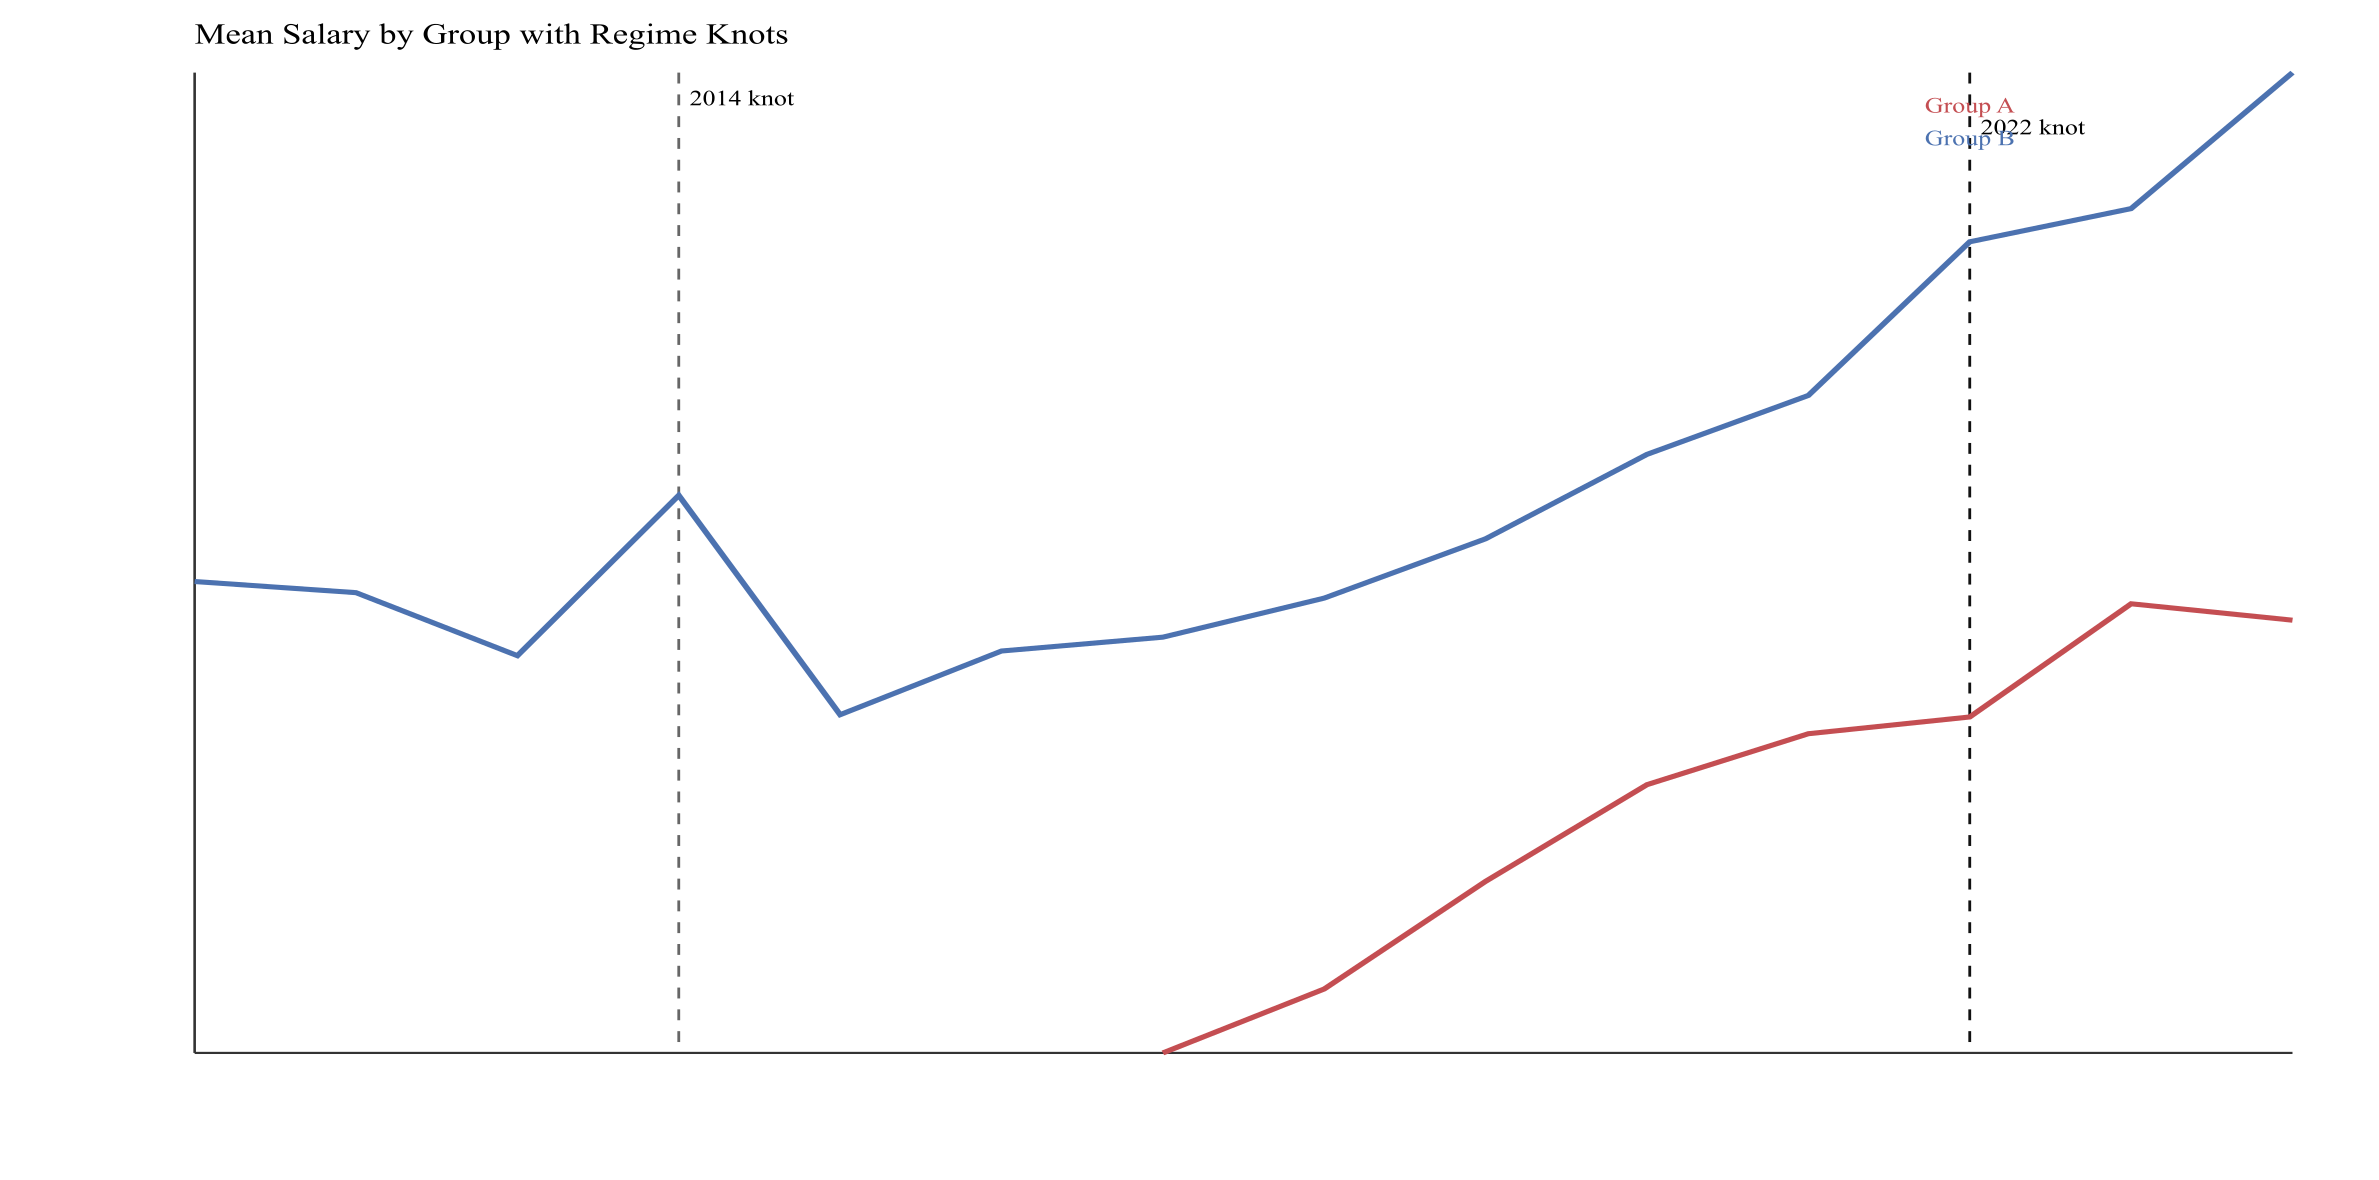
\includegraphics[width=.78\textwidth]{figures/scatter.png}
    \caption{Salary trajectories by group with trend overlays (descriptive only).}
    \label{fig:salary_trajectories}
\end{figure}
}{}

\IfFileExists{figures/salary_boxplot_by_group.png}{
\begin{figure}[h]
    \centering
    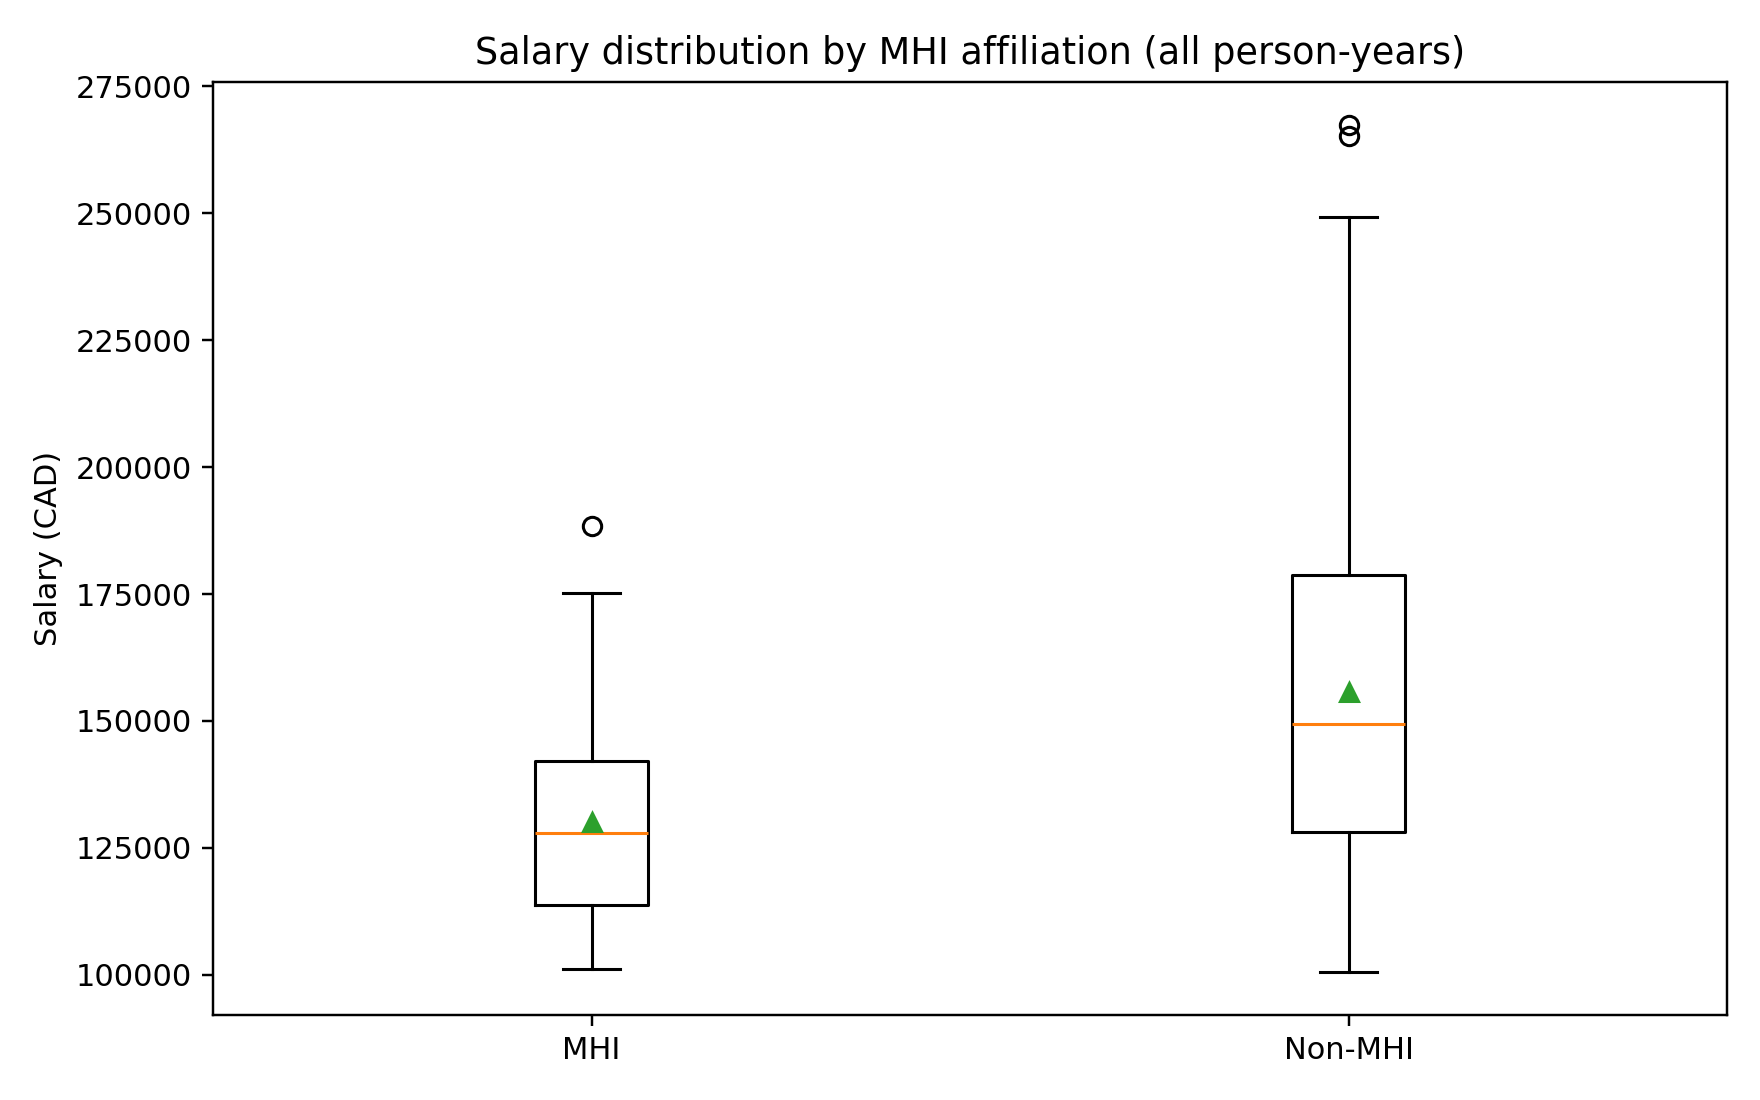
\includegraphics[width=.68\textwidth]{figures/salary_boxplot_by_group.png}
    \caption{Salary distribution comparison by group (boxplots; descriptive only).}
    \label{fig:salary_boxplot}
\end{figure}
}{
\textit{Boxplot figure not found in this environment; descriptive table and trajectory figure are available.}
}

This section is descriptive only.

\section{5. Empirical Strategy}

\subsection*{5.1 Model A --- Salary Level Differences}
\[
salary_{it} = \alpha_i + \beta_1 year_t + \beta_2 group_i + \epsilon_{it}
\]

\begin{itemize}[leftmargin=*]
    \item Person fixed effects and cluster-robust standard errors are preferred where identifiable.
    \item Identification note: because \(group_i\) is time-invariant, \(\beta_2\) is absorbed under strict person FE. The reported level contrast is therefore estimated from pooled OLS as a complementary level-difference model.
\end{itemize}

\subsection*{5.2 Model B --- Salary Growth Differences}
\[
salary_{it} = \alpha_i + \beta_1 year_t + \beta_2 (year_t \times group_i) + \epsilon_{it}
\]

\begin{itemize}[leftmargin=*]
    \item The interaction term \(\beta_2\) measures differential annual growth.
    \item This contrast is identified in both pooled and person-FE specifications.
\end{itemize}

\subsection*{5.3 Small-Sample Inference}
\begin{itemize}[leftmargin=*]
    \item Permutation/randomization test:
    \item Group labels are shuffled across faculty clusters.
    \item The target coefficient is recomputed per shuffle.
    \item The observed estimate is compared with the permutation distribution (two-sided tail area).
    \item Bootstrap confidence intervals are planned but not yet implemented in the current repository version.
    \item Given sample size, conclusions emphasize magnitude and interval uncertainty, not thresholded significance.
\end{itemize}

\subsection*{5.4 Segmented Growth Model (Pre-specified Knots)}
To capture leadership-regime changes without cherry-picking a single break year, we estimate a parsimonious two-knot piecewise-linear growth model with knots at 2014 and \(k_2\), where \(k_2\) defaults to 2022 and is varied in sensitivity analyses (\(k_2 \in \{2021, 2022, 2023\}\)).

Define hinge terms:
\[
k_{2014,t} = \max(0, year_t - 2014), \quad k_{k_2,t} = \max(0, year_t - k_2).
\]

The pooled segmented model is:
\[
salary_{it} = \beta_0 + \beta_1 year_{c,t} + \beta_2 k_{2014,t} + \beta_3 k_{k_2,t}
+ \beta_4 group_i + \beta_5 (year_{c,t}\times group_i)
+ \beta_6 (k_{2014,t}\times group_i) + \beta_7 (k_{k_2,t}\times group_i) + \epsilon_{it}.
\]

The preferred person fixed-effects version drops time-invariant terms absorbed by \(\alpha_i\):
\[
salary_{it} = \alpha_i + \beta_1 year_{c,t} + \beta_2 k_{2014,t} + \beta_3 k_{k_2,t}
+ \beta_5 (year_{c,t}\times group_i) + \beta_6 (k_{2014,t}\times group_i)
+ \beta_7 (k_{k_2,t}\times group_i) + \epsilon_{it}.
\]

Key segmented contrast parameters are \(\phi_{2014}=\beta_6\) and \(\phi_{k_2}=\beta_7\), interpreted as changes in the MHI-minus-non-MHI growth gap after each knot. Cluster-level permutation tests are applied to both \(\phi_{2014}\) and \(\phi_{k_2}\), using the same label-shuffling scheme as the main models.

\section{6. Results}

\subsection*{6.1 Salary Level Differences}

Estimated pooled level difference at centered year is \(+\$14{,}213\) (95\% CI: \([-\$27{,}775,\ +\$56{,}201]\)); permutation p-value is 0.631. Magnitude is potentially meaningful but highly uncertain.

\subsection*{6.2 Salary Growth Differences}

Growth-difference estimates are \(-\$720\)/year (pooled, 95\% CI: \([-\$6{,}593,\ +\$5{,}154]\), permutation p-value 0.833) and \(-\$929\)/year (person FE, 95\% CI: \([-\$3{,}028,\ +\$1{,}170]\), permutation p-value 0.476). Point estimates are consistently negative, but precision is limited.

\IfFileExists{analysis_output/regression_summary.csv}{
\begin{table}[h]
    \centering
    \small
    \resizebox{\textwidth}{!}{
    \pgfplotstabletypeset[
        col sep=comma,
        string type,
        columns={model,term,estimate,std_error,ci_lower,ci_upper,n_obs,n_clusters},
        columns/model/.style={column name=Model},
        columns/term/.style={column name=Term},
        columns/estimate/.style={column name=Estimate},
        columns/std_error/.style={column name=SE},
        columns/ci_lower/.style={column name=CI Low},
        columns/ci_upper/.style={column name=CI High},
        columns/n_obs/.style={column name=N},
        columns/n_clusters/.style={column name=Clusters},
        every head row/.style={before row=\toprule,after row=\midrule},
        every row no 4/.style={after row=\addlinespace},
        every last row/.style={after row=\bottomrule}
    ]{analysis_output/regression_summary.csv}
    }
    \caption{Regression estimates for level and growth contrasts.}
    \label{tab:level_growth_main}
\end{table}
}{
\textit{Regression summary CSV not found. Run the SalaryData executable.}
}

\IfFileExists{analysis_output/permutation_inference_summary.csv}{
\begin{table}[h]
    \centering
    \small
    \resizebox{\textwidth}{!}{
    \pgfplotstabletypeset[
        col sep=comma,
        string type,
        columns={model,term,observed_estimate,ci_lower,ci_upper,p_two_sided,n_permutations,inference_method,n_clusters,n_treated_clusters},
        columns/model/.style={column name=Model},
        columns/term/.style={column name=Term},
        columns/observed_estimate/.style={column name=Observed},
        columns/ci_lower/.style={column name=CI Low},
        columns/ci_upper/.style={column name=CI High},
        columns/p_two_sided/.style={column name=Permutation p},
        columns/n_permutations/.style={column name=Shuffles},
        columns/inference_method/.style={column name=Method},
        columns/n_clusters/.style={column name=Clusters},
        columns/n_treated_clusters/.style={column name=Treated Clusters},
        every head row/.style={before row=\toprule,after row=\midrule},
        every last row/.style={after row=\bottomrule}
    ]{analysis_output/permutation_inference_summary.csv}
    }
    \caption{Permutation inference for level and growth contrasts.}
    \label{tab:perm_main}
\end{table}
}{
\textit{Permutation summary CSV not found. Run the SalaryData executable.}
}

\subsection*{6.3 Sensitivity Analyses}
\begin{itemize}[leftmargin=*]
    \item Terminal-degree-domain exploratory model (private CV-coded subset) was estimated; effects were unstable across pooled and FE specifications.
    \item Outlier exclusion, inflation adjustment, and additional subsample checks are not yet implemented in the current version.
\end{itemize}

\subsection*{6.4 Segmented Growth Results}
\IfFileExists{analysis_output/segmented_model_summary.csv}{
\begin{table}[h]
    \centering
    \small
    \resizebox{\textwidth}{!}{
    \pgfplotstabletypeset[
        col sep=comma,
        string type,
        columns={breakYear,model,preGrowthGap,after2014GrowthGap,afterK2GrowthGap,phi2014,phiK2,phi2014SE,phiK2SE},
        columns/breakYear/.style={column name=Knot2 Year},
        columns/model/.style={column name=Model},
        columns/preGrowthGap/.style={column name=Gap Pre-2014},
        columns/after2014GrowthGap/.style={column name=Gap 2014--(Knot2-1)},
        columns/afterK2GrowthGap/.style={column name=Gap Knot2+},
        columns/phi2014/.style={column name=\(\phi_{2014}\)},
        columns/phiK2/.style={column name=\(\phi_{k_2}\)},
        columns/phi2014SE/.style={column name=SE(\(\phi_{2014}\))},
        columns/phiK2SE/.style={column name=SE(\(\phi_{k_2}\))},
        every head row/.style={before row=\toprule,after row=\midrule},
        every last row/.style={after row=\bottomrule}
    ]{analysis_output/segmented_model_summary.csv}
    }
    \caption{Two-knot segmented growth model estimates (pooled and person FE).}
    \label{tab:segmented_main}
\end{table}
}{
\textit{Segmented model summary CSV not found. Run the SalaryData executable.}
}

\IfFileExists{analysis_output/segmented_permutation_summary.csv}{
\begin{table}[h]
    \centering
    \small
    \resizebox{\textwidth}{!}{
    \pgfplotstabletypeset[
        col sep=comma,
        string type,
        columns={breakYear,model,term,observed,pTwoSided,nPermutations,inferenceMethod},
        columns/breakYear/.style={column name=Knot2 Year},
        columns/model/.style={column name=Model},
        columns/term/.style={column name=Term},
        columns/observed/.style={column name=Observed},
        columns/pTwoSided/.style={column name=Permutation p},
        columns/nPermutations/.style={column name=Shuffles},
        columns/inferenceMethod/.style={column name=Method},
        every head row/.style={before row=\toprule,after row=\midrule},
        every last row/.style={after row=\bottomrule}
    ]{analysis_output/segmented_permutation_summary.csv}
    }
    \caption{Permutation inference for segmented contrasts \(\phi_{2014}\) and \(\phi_{k_2}\).}
    \label{tab:segmented_perm}
\end{table}
}{}

\section{7. Power and Detectable Effects}

A rough minimum-detectable-effect (MDE) approximation uses \((1.96 + 0.84)\times SE \approx 2.8\times SE\):
\begin{itemize}[leftmargin=*]
    \item Level contrast MDE (pooled): about \(\$60{,}000\).
    \item Growth contrast MDE (pooled): about \(\$8{,}391\)/year.
    \item Growth contrast MDE (person FE): about \(\$2{,}998\)/year.
\end{itemize}

This implies null findings are compatible with both ``no effect'' and ``effects smaller than current precision allows us to detect reliably.''

\section{8. Limitations}
\begin{itemize}[leftmargin=*]
    \item No access to internal merit or promotion timing.
    \item No rank-level controls in the primary models.
    \item Small departmental sample.
    \item Observational design and potential omitted-variable bias.
\end{itemize}

\section{9. Interpretation}

Point estimates for growth differences are consistently negative, and the implied practical gap over multi-year horizons may be meaningful. At the same time, uncertainty remains substantial and permutation results are not extreme under the null. Stronger conclusions require richer covariates and additional sample depth.

\section{10. Conclusion}
\begin{enumerate}[leftmargin=*]
    \item What the data show: directionally negative growth contrasts for Group A relative to Group B, with wide uncertainty.
    \item What the data do not show: definitive evidence of persistent level or growth differences at current precision.
    \item What additional data would clarify the issue: promotion timing, rank/history, workload, and extended longitudinal coverage.
\end{enumerate}

\appendix

\section{Appendix A: Full Regression Tables}

Table~\ref{tab:level_growth_main} and Table~\ref{tab:perm_main} provide the full model outputs used in the main text.

\section{Appendix B: Permutation Distribution Summaries}

\IfFileExists{analysis_output/permutation_inference_summary.csv}{
\begin{table}[h]
    \centering
    \small
    \resizebox{\textwidth}{!}{
    \pgfplotstabletypeset[
        col sep=comma,
        string type,
        columns={model,term,null_mean,null_std_dev,null_q025,null_q975,n_permutations},
        columns/model/.style={column name=Model},
        columns/term/.style={column name=Term},
        columns/null_mean/.style={column name=Null Mean},
        columns/null_std_dev/.style={column name=Null SD},
        columns/null_q025/.style={column name=Null 2.5\%},
        columns/null_q975/.style={column name=Null 97.5\%},
        columns/n_permutations/.style={column name=Shuffles},
        every head row/.style={before row=\toprule,after row=\midrule},
        every last row/.style={after row=\bottomrule}
    ]{analysis_output/permutation_inference_summary.csv}
    }
    \caption{Permutation distribution summaries.}
    \label{tab:perm_distribution_summary}
\end{table}
}{}

\section{Appendix C: Data Cleaning Documentation}
\begin{itemize}[leftmargin=*]
    \item Faculty names are canonicalized before merges across salary and cohort lists.
    \item Group labels are assigned from the public Health Informatics roster for Group A.
    \item Panel remains unbalanced; missing salary years are not imputed.
    \item Local/private CV-based files are excluded from git and used only for local exploratory covariates.
\end{itemize}

\section{Appendix D: Code Repository}

\url{https://github.com/JimWallace/SPHS-Salary-Analysis---2024}

\section{Appendix E: Faculty-Level Exploratory Matrix}
\label{app:faculty_exploratory_matrix}

\IfFileExists{analysis_output/appendix_faculty_exploratory_matrix.csv}{
\clearpage
\begin{landscape}
\begin{table}[p]
    \centering
    \scriptsize
    \setlength{\tabcolsep}{2.4pt}
    \renewcommand{\arraystretch}{1.05}
    \resizebox{\linewidth}{!}{
    \pgfplotstabletypeset[
        col sep=comma,
        string type,
        columns={
            faculty_name,mhi,term_domain,term_non_health,term_reason_code,self_parse_status,self_text_quality,
            sf_health_services_policy,sf_mental_behavioral,sf_epidemiology_biostatistics,sf_aging_gerontology,
            sf_rehabilitation_disability,sf_substance_tobacco,sf_environmental_occupational,sf_nutrition_diet,
            sf_health_informatics_data,sf_global_population_health,public_listed,public_cross_appointment,
            public_group_count,g_researchers,g_cdpm,g_health_policy,g_health_aging,g_health_environment,g_food_water,
            g_hi,g_global_health,g_neuro_cog_epi,g_healthy_workplaces
        },
        columns/faculty_name/.style={column name=Faculty},
        columns/mhi/.style={column name=MHI},
        columns/term_domain/.style={column name=TDomain},
        columns/term_non_health/.style={column name=TNonHlth},
        columns/term_reason_code/.style={column name=TReason},
        columns/self_parse_status/.style={column name=SParse},
        columns/self_text_quality/.style={column name=SQuality},
        columns/sf_health_services_policy/.style={column name=SF\_HSP},
        columns/sf_mental_behavioral/.style={column name=SF\_MB},
        columns/sf_epidemiology_biostatistics/.style={column name=SF\_EPI},
        columns/sf_aging_gerontology/.style={column name=SF\_AGE},
        columns/sf_rehabilitation_disability/.style={column name=SF\_REHAB},
        columns/sf_substance_tobacco/.style={column name=SF\_SUB},
        columns/sf_environmental_occupational/.style={column name=SF\_ENV},
        columns/sf_nutrition_diet/.style={column name=SF\_NUT},
        columns/sf_health_informatics_data/.style={column name=SF\_HI},
        columns/sf_global_population_health/.style={column name=SF\_GLOBAL},
        columns/public_listed/.style={column name=PubList},
        columns/public_cross_appointment/.style={column name=CrossAppt},
        columns/public_group_count/.style={column name=PubN},
        columns/g_researchers/.style={column name=G\_Res},
        columns/g_cdpm/.style={column name=G\_CDPM},
        columns/g_health_policy/.style={column name=G\_Pol},
        columns/g_health_aging/.style={column name=G\_Age},
        columns/g_health_environment/.style={column name=G\_Env},
        columns/g_food_water/.style={column name=G\_Food},
        columns/g_hi/.style={column name=G\_HI},
        columns/g_global_health/.style={column name=G\_Global},
        columns/g_neuro_cog_epi/.style={column name=G\_Neuro},
        columns/g_healthy_workplaces/.style={column name=G\_Work},
        every head row/.style={before row=\toprule,after row=\midrule},
        every last row/.style={after row=\bottomrule}
    ]{analysis_output/appendix_faculty_exploratory_matrix.csv}
    }
    \caption{One-row-per-faculty exploratory matrix combining local CV-derived indicators and public SPHS group/cross-appointment fields.}
    \label{tab:faculty_exploratory_matrix}
\end{table}
\end{landscape}
\clearpage
}{
\textit{Faculty exploratory matrix CSV not found.}
}

\newpage
\printbibliography

\end{document}
